\newpage
\section{Hardware}
In this chapter we give a short oversight what hardware is used and how big the price tag of the demonstrator is. 

\subsection{Back-light}
The backlight consists of three glass panels of the size 2mm x 600mm x 
\begin{figure}[ht]
	\centering
	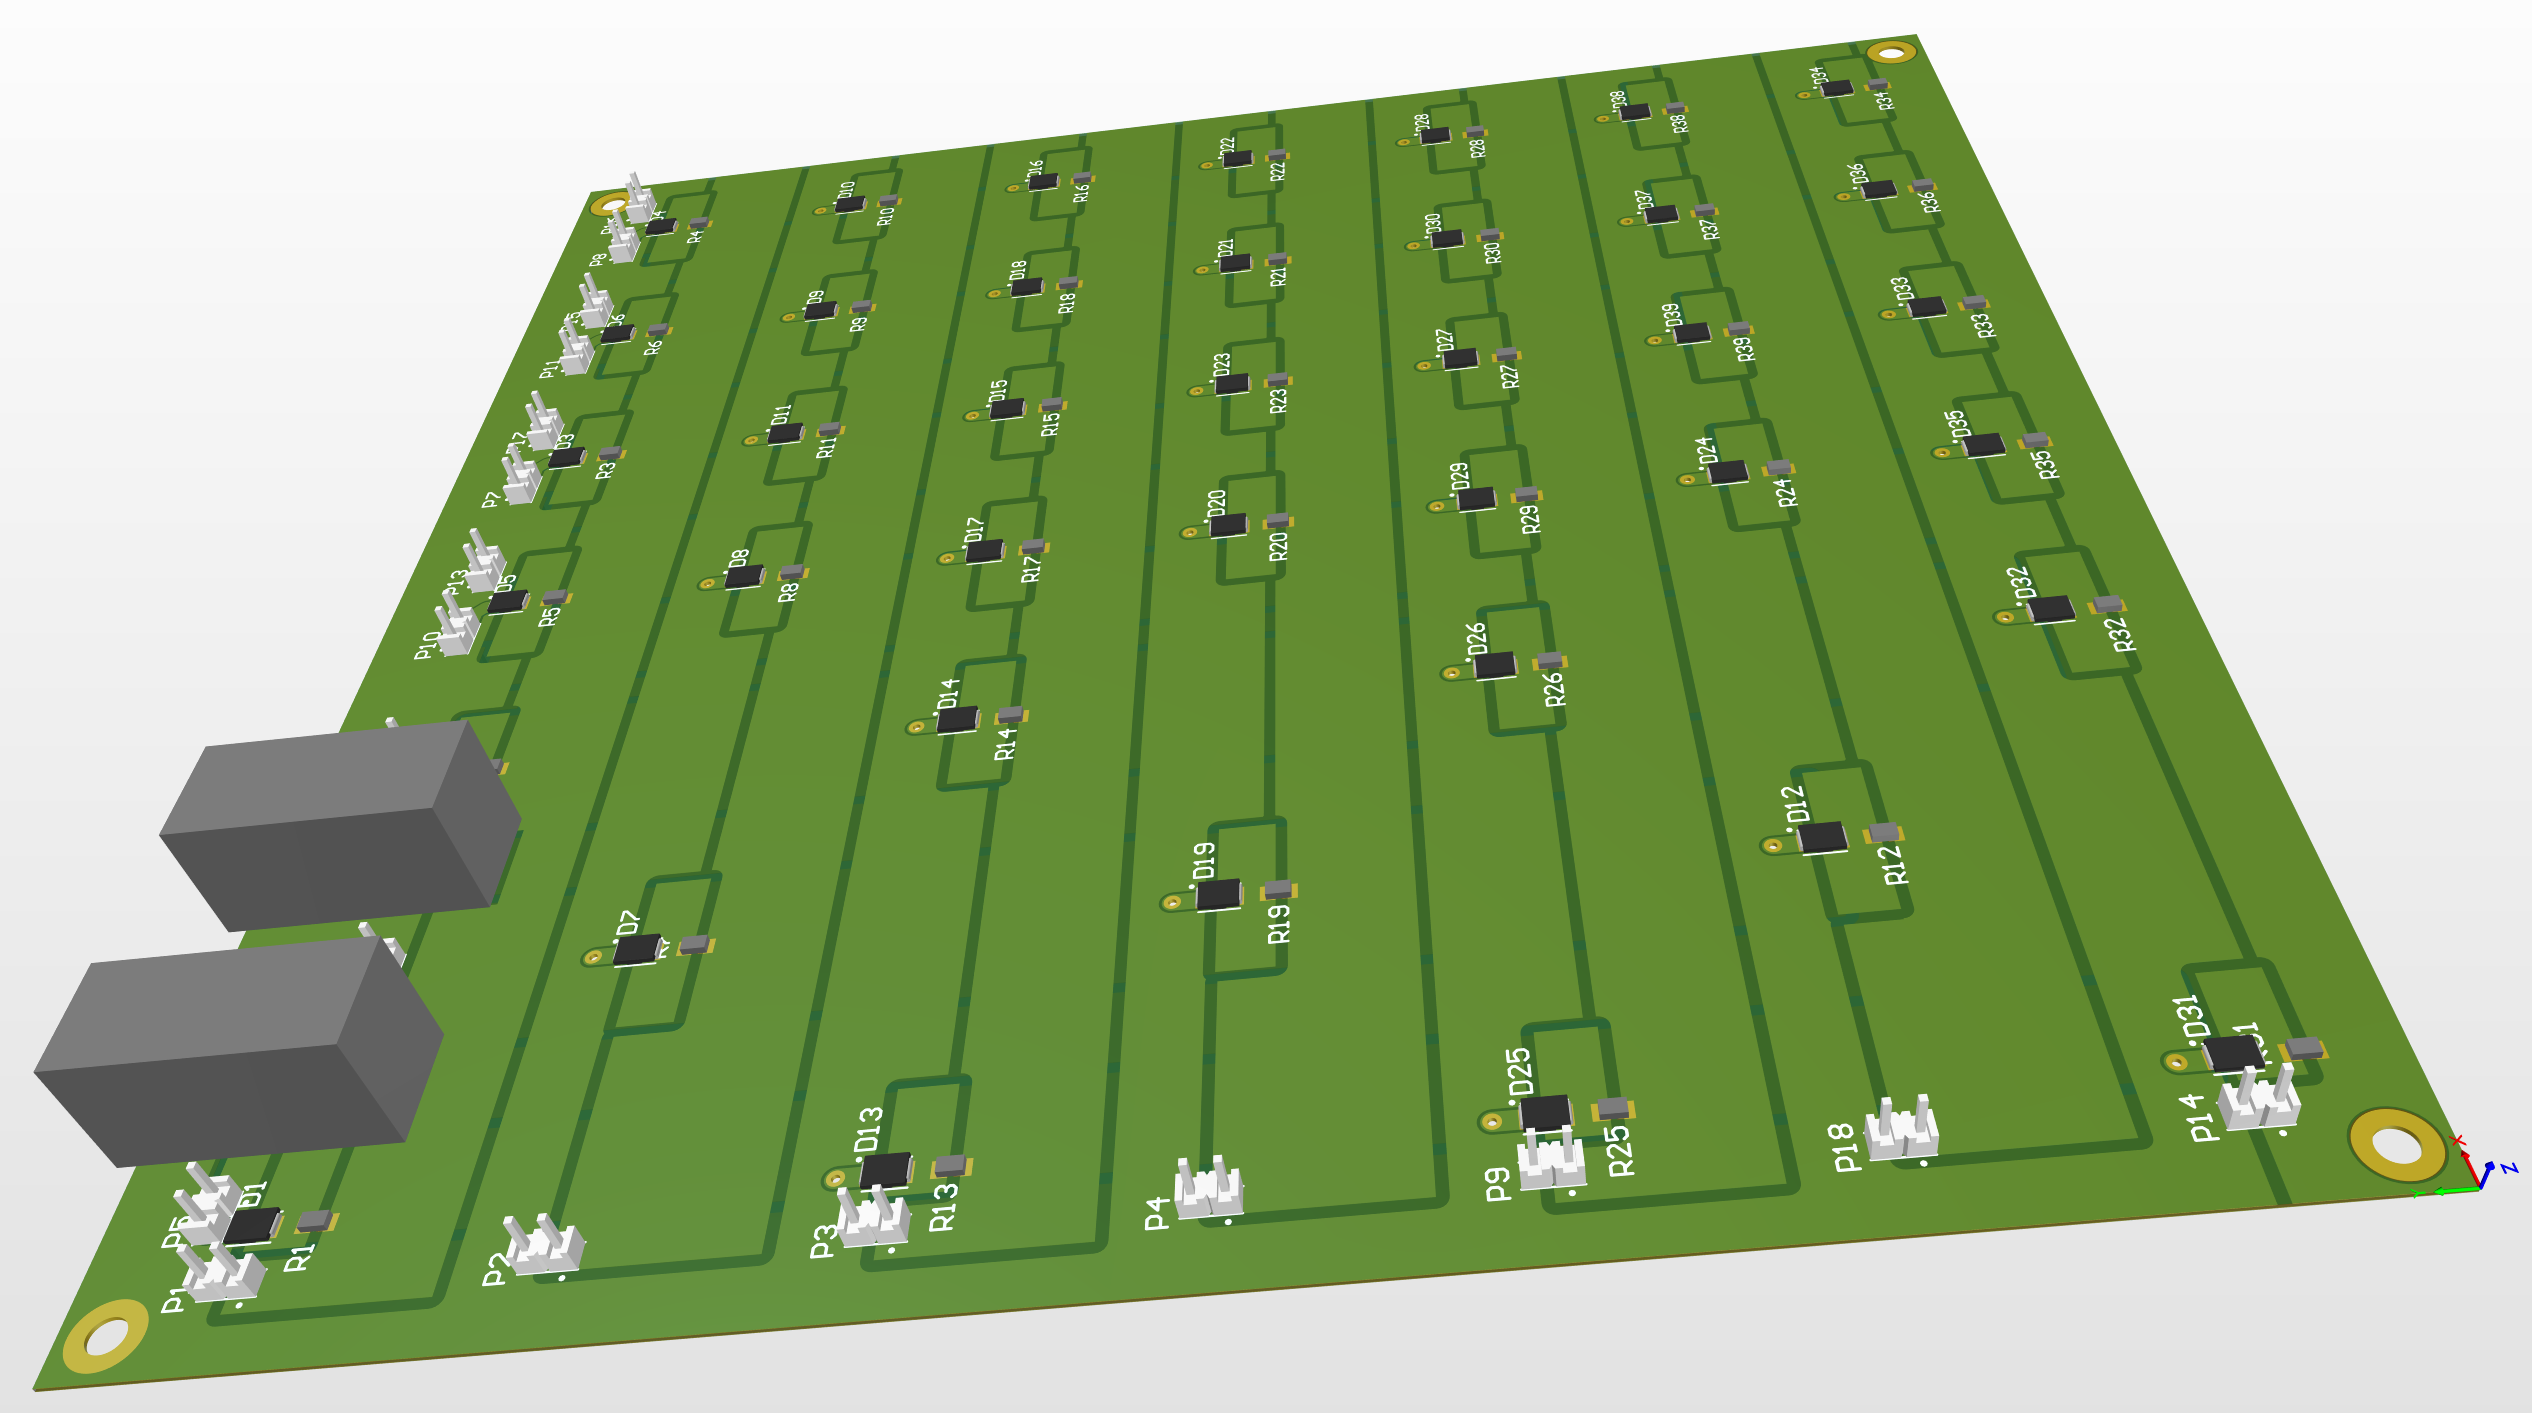
\includegraphics[width=0.9\textwidth]{3-development/images/Backlight.png}
	\caption{3D-Model of the back-light PCB\label{development:pcb}}
\end{figure} 

\subsection{Computer}
The computer used is the Jetson Nano Developer Kit. a short technical overview of the Jetson Nano taken from the official website:https://developer.nvidia.com/embedded/jetson-nano-developer-kit \textbf{Ref}\\

\begin{tabular}{ |l c|  }
	\hline
	\multicolumn{2}{|c|}{Technical specifications of the Jetson Nano} \\
	\hline
	GPU			& 	128-core Maxwell\\
	CPU			& 	Quad-core ARM A57 @ 1.43 GHz \\
	Memory 		&	4 GB 64-bit LPDDR4 25.6 GB/s 				\\
	Storage		&	microSD				\\
	Video Encode&	4K @ 30 | 4x 1080p @ 30 | 9x 720p @ 30 (H.264/H.265) \\
	Video Decode&	4K @ 60 | 2x 4K @ 30 | 8x 1080p @ 30 | 18x 720p @ 30 (H.264/H.265) \\
	Camera 		&	2x MIPI CSI-2 DPHY lanes \\
	Connectivity&	Gigabit Ethernet, M.2 Key E\\
	Display 	&	HDMI and display port \\
	USB 		&	4x USB 3.0, USB 2.0 Micro-B\\
	Others 		&	GPIO, I2C, I2S, SPI, UART \\
	Mechanical 	&	69 mm x 45 mm, 260-pin edge connector \\
	
	\hline
\end{tabular}


\subsection{Camera}
The camera used for this project had to following evaluation criteria to meet:
\begin{itemize}
	\item Compatible with the Jetson Nano enviroment
	\item A good developer community
	\item Open source drivers
	\item Low cost
\end{itemize}

Table \ref{development:cameras} lists some of the cameras that have been evaluated for the project.
\begin{table}[ht]
	\centering
	\begin{tabular}{ |l||c|c|c|  }
		\hline
		\multicolumn{4}{|c|}{List of possible Cameras} \\
		\hline\hline
		Company				& Raspberry Pi 		& Raspberry Pi	& Arducam\\
		Camera Name			& Camera Module V2 	& HQ Camera		& Arducam IMX219 \\
		&					&				&Low Distortion M12 \\
		&					&				&Mount Camera Module\\
		\hline
		Price				& \$25 				& \$50  		& \$39.99 \\
		Camera Sensor   	& Sony IMX219 		& Sony IMX477	& Sony IMX219\\
		
		Still resolution	& 8M 				& 12M			& 12.3M\\
		Sensor resolution 	& 3280 x 2464 		& 4056 x 3040 	& 3280 x 2464\\
		Linux integration   & V4L2 driver 		& V4L2 driver	& V4L2 driver\\
		Pixel size			& 1.12 x 1.12 $\mu\text{m}$	& 1.55 x 1.55$\mu\text{m}$ & 1.12 x 1.12 $\mu\text{m}$ \\
		Focal length		& 3.04$[\text{mm}]$ & Depends on lens & 2.8$[\text{mm}]$\\
		Focal ratio			& 2.0  				& Depends on lens & 2.8\\
		View angle Horizontal & 62.2 deg.		& Depends on lens & 75 deg.\\
		\hline
	\end{tabular}
\caption{List of suitable cameras.\label{development:cameras}}	
\end{table}

In the end, all results were measured with the Raspberry Pi Camera Module V2 since it was the cheapest one in the list and seems to deliver the desired results.

\subsection{Demonstrator}
The demonstrator consists of three essential components. The framework that holds everything together, the backlight that illuminates from bottom to top and the Jetson nano with a camera. The Jetson nano is mounted on a 3d printed mount together with the camera. The camera is pointed directly at the backlight.  \\
The framework consists of 15 aluminum profiles which are all bolted together with angles. The framework is also by far the most expensive component of the entire prototype with xxx. 

\begin{figure}[ht]
	\centering
	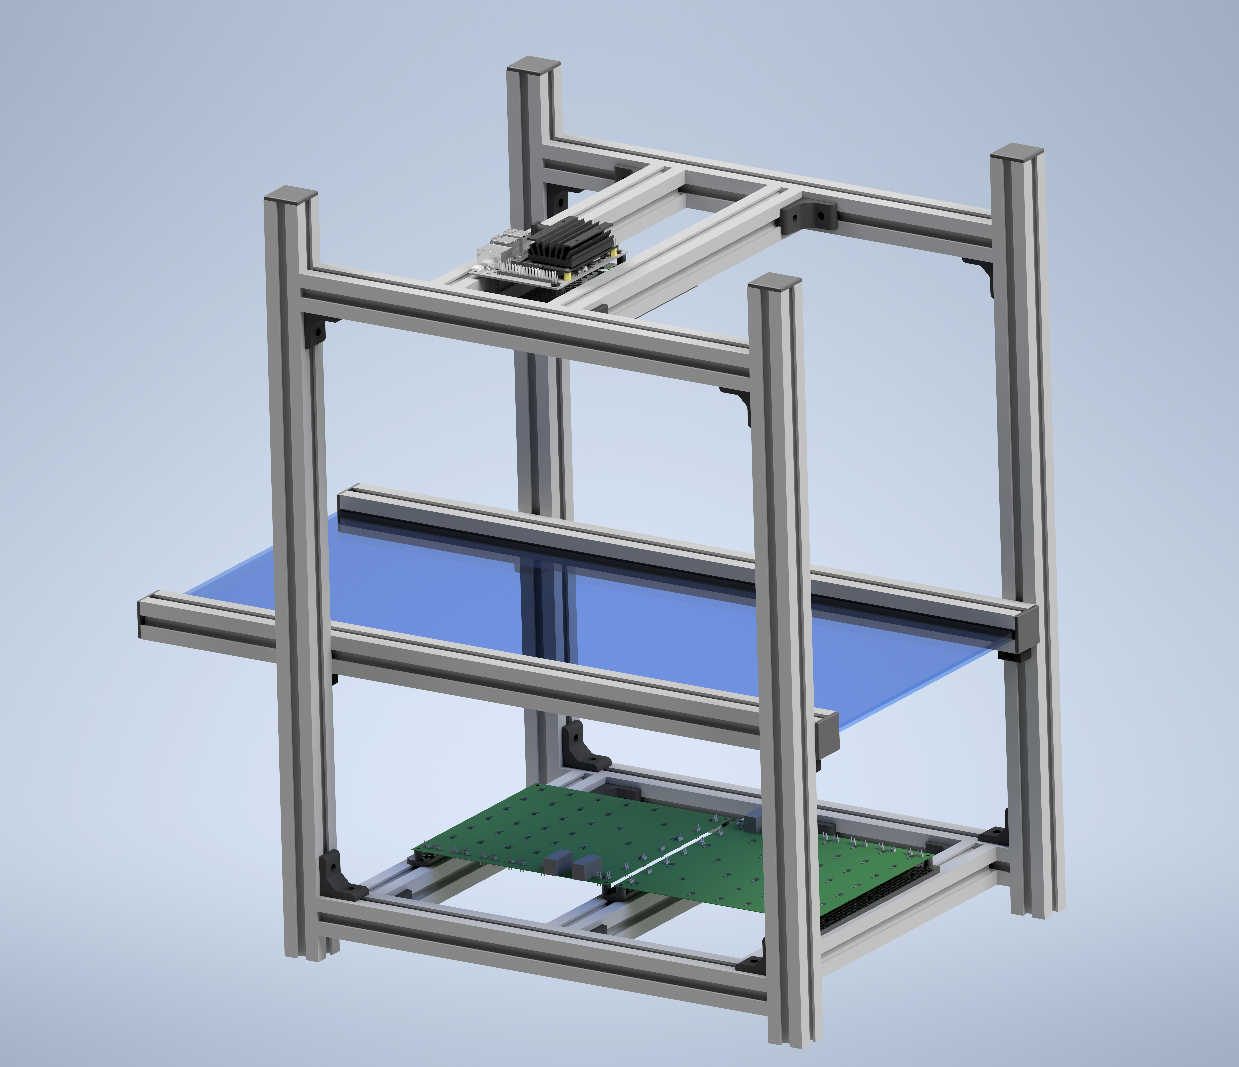
\includegraphics[width=0.9\textwidth]{3-development/images/Demonstrator.png}
	\caption{3D-Model of the demonstrator\label{development:demo}}
\end{figure} 
\newpage

\subsection{Production cost}
The cost of one demonstrator unit listed.\\

\begin{tabular}{|l|c|c|c|}
	\hline
	Part & quantity & price each& total\\
	\hline
	Mineral glass & 3 & 10.95 & 32.85\\
	\hline
\end{tabular}

The estimated material cost of 1000 units listed.\\

\begin{tabular}{|l|c|c|c|}
	\hline
	Part & quantity & price each& total\\
	\hline
	Mineral glass & 3 & 10.95 & 32.85\\
	\hline
\end{tabular}